\documentclass[margin=3mm]{standalone} 
\usepackage{tikz}
\usetikzlibrary{shapes.geometric}
\begin{document}
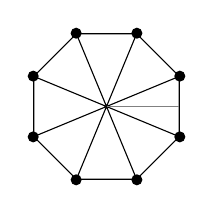
\begin{tikzpicture}[dot/.style={circle,fill,inner sep=0pt,minimum size=4pt}]
 \draw node[regular polygon,regular polygon sides=8,draw,minimum size=2cm]
 (p8){}
  foreach \X[count=\Y] in {5,...,8} {(p8.corner \X) node[dot](n-\X){}
    -- (p8.corner \Y) node[dot](n-\Y){} };
\draw [gray] (0mm,0mm) -- (0.915cm,0);
\end{tikzpicture}
\end{document}